\documentclass{article} 
\usepackage[danish]{babel} 
\usepackage[utf8]{inputenc}
\usepackage{float} 
\usepackage{fancyhdr} 
\usepackage{amsmath} 
\usepackage[usenames,dvipsnames]{color}
\usepackage{listingsutf8} 
\usepackage{listings} 
\usepackage{graphicx} 
\usepackage{pdfpages}
\usepackage{booktabs} %
\usepackage{enumitem}
\lstset{language=R,basicstyle=
  \ttfamily\small} \title{Statistik og dataanalyse
\\ Tællende aktivitet 1} 
\author{Peter Heilbo Ratgen - perat17@student.sdu.dk}
\date{ \today} 

  \lstset{ 
  language=R,                     % the language of the code
  basicstyle=\small\ttfamily, % the size of the fonts that are used for the code
  numbers=left,                   % where to put the line-numbers
  numberstyle=\tiny\color{Blue},  % the style that is used for the line-numbers
  stepnumber=1,                   % the step between two line-numbers.  If it is 1, each line
  % will be numbered
  numbersep=5pt,                  % how far the line-numbers are from the code
  showspaces=false,               % show spaces adding particular underscores
  showstringspaces=false,         % underline spaces within strings
  showtabs=false,                 % show tabs within strings adding particular underscores
  frame=single,                   % adds a frame around the code
  rulecolor=\color{black},        % if not set, the frame-color may be changed on line-breaks within not-black text (e.g. commens (green here))
  tabsize=2,                      % sets default tabsize to 2 spaces
  captionpos=b,                   % sets the caption-position to bottom
  breaklines=true,                % sets automatic line breaking
  breakatwhitespace=false,        % sets if automatic breaks should only happen at whitespace
  keywordstyle=\color{RoyalBlue},      % keyword style
  commentstyle=\color{YellowGreen},   % comment style
  stringstyle=\color{ForestGreen}      % string literal style
} 

\begin{document} 
\maketitle 
\newpage 
\section{Databehandling}
Datafilen indeholder data om landes CO2-udledning per indbygger i metriske ton
per indbygger. Der er to kolonner i datafilen, "Country" og "CO2". Først gemmes
.xlsx-filen som en .csv fil. Denne data er dog ikke komplet, det indeholder også
de lande eller territorier der ikke har opgivet data. Det giver ikke mening at
betragte disse lande i statistikken, derfor fjernes disse fra datasættet. Dette
gøres ved at fjerne alle datapunkter der har ".." som værdi.  Også datapunkter
der ikke er lande skal også fjernes fra datasættet, derfor fjernes alle
datapunkter hvor "income" indgår i navnet med kommandolinjeværktøjet
\texttt{sed}. Her er der fjernet 10 datapunkter. Derudover fjernes datapunktet
"world" også, siden det noget der kan regnes frem til. Til sidst i
databehandlingen skal \lstinline|,| ændres til \lstinline|.|, for at R
importerer data som den korrekte type.

Nu kan data indporteres til R med:
\begin{lstlisting}[language=R]
co2  <- read.csv("CO2.csv", sep = ";", row.names = NULL)
\end{lstlisting}
Her bruges \lstinline|sep = ";"| til at indikere at værdierne i .csv formatet
ikke er separeret med et komma, men med et semikolon.

\section{Grafiske illustrationer}

\subsection{Histogram}

\begin{figure}[H]
  \centering
  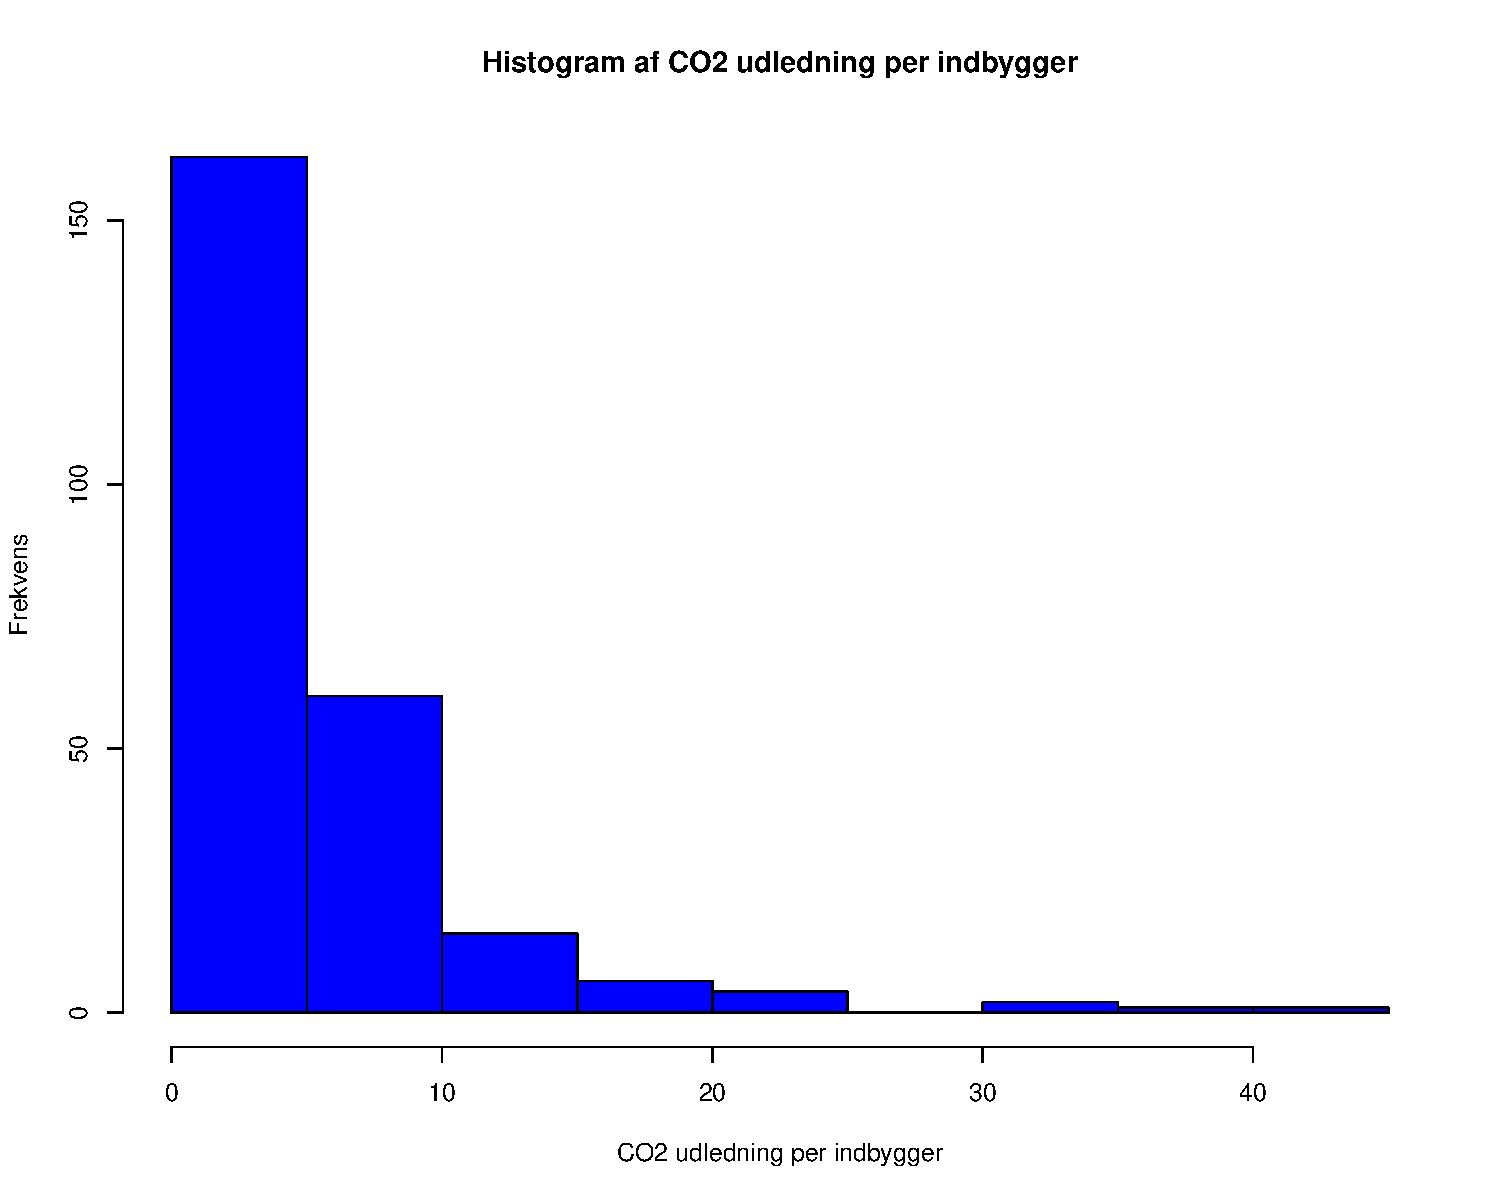
\includegraphics[width=0.8\textwidth]{co2plot.pdf}
\end{figure}

\subsection{Boxplot}

\begin{figure}[H]
  \centering
  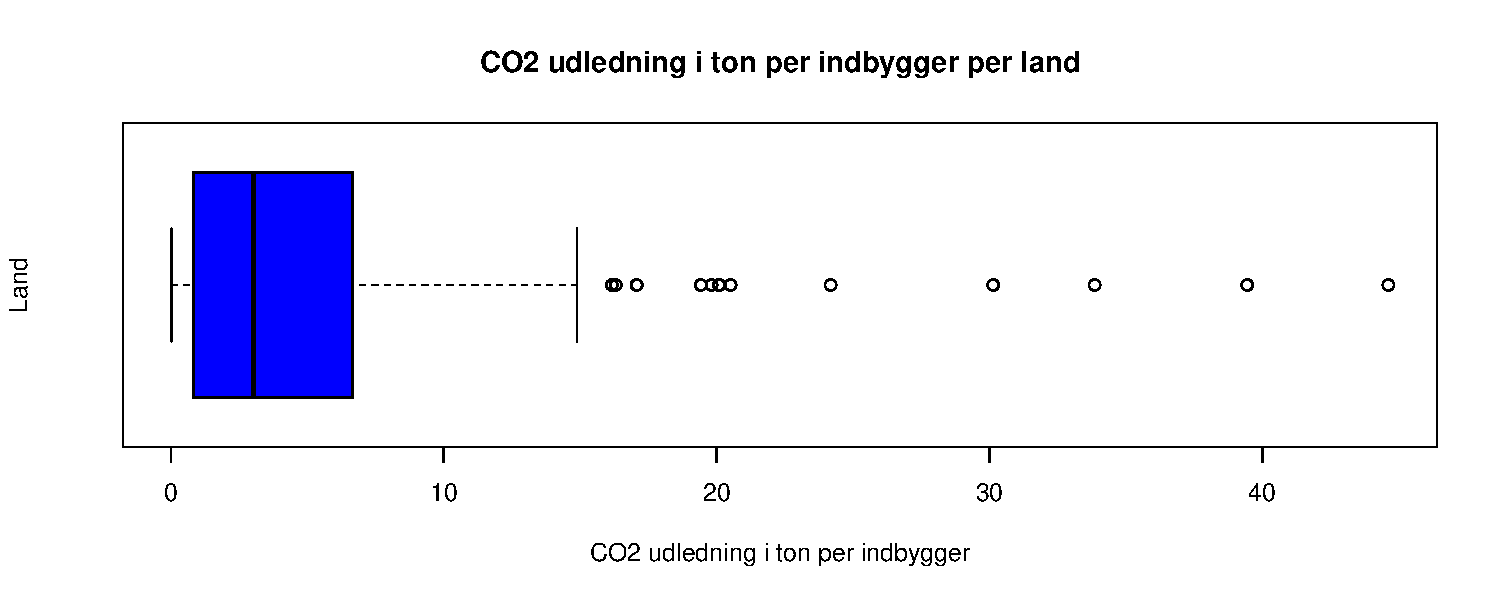
\includegraphics[width=0.9\textwidth]{co2boxplot.pdf}
\end{figure}

Boxplottet fortæller at langt de flest lande (75\%, eller dem inden for det 3.
kvartil) ikke udleder over 10 ton CO2 per indbygger. Det fortæller også at der
er nogle lande der udleder langt mere CO2 per indbygger, disse er de lande der
ligger uden for 1.5 gange den interkvatile afstand.

Danmark ligger indenfor det 3. kvartil med sine 6.51 ton CO2 udledt per
indbygger. Det vil også sige at Danmark ligger over medianen.

\section{Deskriptiv analyse}
\begin{table}[H]
  \begin{tabular}{l|l}
    Gennemsnit        & 4.9489  \\\hline
    Median            & 3.0259  \\\hline
    Typeinterval      & 0-5 \\\hline
    Standardafvigelse & 6.1881  \\\hline
    Standard error    & 0.0246  \\\hline
    Varians           & 38.2931 \\\hline
    Minimum           & 0.0303  \\\hline
    Maximum           & 44.6179 \\\hline
    $Q_1$             & 0.8280  \\\hline
    $Q_3$             & 6.6646 
  \end{tabular}
\end{table}

\section{Normalfordeling}
Som det ses på ovenstående histogram er data er højreskæv. Normalfordelingen har
en symmetrisk klokkeform. En anden indikator er at gennemsnittet og medianen
ikke er tæt på at være den samme værdi.

Derfor er data ikke normalfordelt.

\newpage
\section{R-kode}
\lstinputlisting[language=R,inputencoding=utf8/latin1]{aktivitet.R}

\end{document}
